\chapter{Beam Use Proposal 2026-2027}
\label{chap:beam_use_proposal_extra}

In this Chapter we provide details on a potential additional two years of running in 2026-2027 that presents a further return on investment in sPHENIX and also the entire RHIC program.   We highlight if such a window of opportunity arises this would represent the last opportunity for data taking in heavy-ion mode in this energy regime in our lifetime. 

\section{Proposal Summary}

The sPHENIX proposal for such a potential window of opportunity is summarized in Table~\ref{tab:summary2627}.   The two years assume 28 cryo-weeks in each and with a sPHENIX uptime of 80\% with detector operations having reached a mature state.   Projected luminosities are documented by these years 2026 and 2027 by C-AD.  For completeness we detail in the cryo-weeks for the potential 2026 and 2027 runs at the end of this Chapter in Section~\ref{sec:cryo20262027}.

\begin{table}[h]
\centering
\caption{The recorded luminosity (Rec. Lum.) and sampled luminosity (Samp. Lum.) values are for collisions with z-vertex $|z|<$ 10 cm.  \label{tab:summary2627}}
\bigskip
\centering
\begin{tabular}{ | c | c | c | c | c | c | c  | }
\hline
Year & Species & $\sqrt{s_{NN}}$ & Cyro  & Physics & Rec. Lum. & Samp. Lum. \\
     &         & [GeV]           & Weeks & Weeks   & $|z|<$10~cm & $|z|<$10~cm  \\ \hline \hline
     {\bf 2026} & $p^{\uparrow}p^{\uparrow}$   & 200 & 28 & 15.5      & 1.0 \pb [10 kHz]   & 130 \pb \\ 
      & & & & & 130~\pb [100\%-$str$] & \\ \hline
 --  & O+O    & 200 & -- & 2        & 14~\nb +  47~\nb [100\%-$str$] & 47~\nb  \\ \hline
 --  & Ar+Ar   & 200 & -- & 2      & 30~\nb + 68~\nb [100\%-$str$] & 68~\nb  \\ \hline \hline
{\bf{2027}} & \auau   & 200 & 28 & 24.5 & 30 \nb [100\%-$str$/DeMux]   & 31 \nb \\ \hline
\end{tabular}
\end{table}

We highlight that key upgrades at very modest cost are a major factor increasing the physics impact of these additional years of running.   DeMultiplexing the calorimeter readout increases the Level-1 trigger accept rate to 30 kHz, doubling the rate of calorimeter data events.    Increasing the tracking detectors streaming readout to 100\% results in an order of magnitude more data than in the 2024-2025 data taking.    These upgrade options are detailed in Chapter~\ref{chap:readout}.

%\section{Physics Projections}
%We detail the potential physics gain from the 2026 and 2027 running in the following two subsections, focusing %first on the additional \auau and \pp running and then on the novel system O+O and Ar+Ar running.

\section{\auau and \pp Physics Reach}

First, we start with the \auau increased physics reach.    In Table~\ref{tab:auau2027} we compare directly the \auau recorded and sampled luminosities from the three runs in 2023, 2025, and the potential opportunity in 2027.   The upgrades enable a doubling of the \auau data set to 30 nb$^{-1}$ or equivalently 200 billion \auau events.    These events are a permanent archive of \auau data to be mined for any future analysis once the RHIC machine is not longer running heavy ions.    There are no trigger biases or selections that would preclude any analysis within the acceptance and performance parameters of sPHENIX.

\begin{table}[h]
\centering
\caption{Summary of Au+Au at 200 GeV option sPHENIX Beam Use Proposal.
The recorded luminosity (Rec. Lum.) and first sampled luminosity (Samp. Lum.) values are for collisions with z-vertex $|z|<$ 10 cm.  The final column shows the sampled luminosity for all z-vertex values, relevant for calorimeter only measurements.\label{tab:auau2027}}
\bigskip
\centering
\begin{tabular}{ | c | c | c | c | c | c | c  | }
\hline
Year & Species & $\sqrt{s_{NN}}$ & Cyro  & Physics & Rec. Lum. & Samp. Lum. \\
     &         & [GeV]           & Weeks & Weeks   & $|z|<$10~cm & $|z|<$10~cm  \\ \hline \hline

2023 & \auau   & 200 & 24 (28) & 9 (13) & 3.7 (5.7) \nb   & 4.5 (6.9) \nb  \\ \hline
2025 & \auau   & 200 & 24 (28) & 20.5 (24.5) & 13 (15) \nb   & 21 (25) \nb  \\ \hline
{\bf{2027}} & \auau   & 200 & 28 & 24.5 & 30 \nb [100\%-$str$/DeMux]   & 31 \nb \\ \hline
\end{tabular}
\end{table}

The impact on the \pp data set is even more substantial.   The comparison of running \pp in 2024 and 2026 is shown in Table~\ref{2026pp}.   The striking gain is in the 130~\pb recorded with the tracking detectors via 100\%-$str$ mode, more than a factor of ten over the previous data set.    There are many measurements, particularly in the heavy-flavor and transverse spin (cold QCD) arena where selecting physics triggers are not available and thus the \pp measurements are the statistical limitation in nuclear modification factors.    This enormous data set both for calorimetric jets with 130~\pb additional sampled and for all channels available via the tracking detectors with 130~\pb recorded again represents an immediate opportunity to advance our precision physics knowledge and a permanent archive of data from RHIC.

\begin{table}[h]
\centering
\caption{The recorded luminosity (Rec. Lum.) and sampled luminosity (Samp. Lum.) values are for collisions with z-vertex $|z|<$ 10 cm.  \label{tab:2026pp}}
\bigskip
\centering
\begin{tabular}{ | c | c | c | c | c | c | c  | }
\hline
Year & Species & $\sqrt{s_{NN}}$ & Cyro  & Physics & Rec. Lum. & Samp. Lum. \\
     &         & [GeV]           & Weeks & Weeks   & $|z|<$10~cm & $|z|<$10~cm  \\ \hline \hline
2024 & $p^{\uparrow}p^{\uparrow}$     & 200 & 24 (28) & 12 (16) & 0.3 (0.4) \pb [5 kHz] & 73 (101) \pb  \\
     &                                &     &  & &  7.3 (10.1) \pb [10\%-$str$]&   \\ \hline
     {\bf 2026} & $p^{\uparrow}p^{\uparrow}$   & 200 & 28 & 15.5      & 1.0 \pb [10 kHz]   & 130 \pb \\ 
      & & & & & 130~\pb [100\%-$str$] & \\ \hline
\end{tabular}
\end{table}

WHICH EXAMPLE FIGURES SHOULD WE INCLUDE HERE... AND HOW MANY!

%%%%%%%%%%%%%%%%%%%%%%%%%%%%%%%%%%%%%%%%%%%%%%%%%%%%%%%%%%%%%%%%%%%%%%%%%%%%%
\section{O+O and Ar+Ar Physics Reach}

The RHIC program has a 100\% track record of learning new physics and gaining insights from every novel nuclear species combinations put into collision.    It is a testament to the facility and the constant improvements, including the EBIS source, that have been the lifeblood of the machine.    An opportunity to run smaller symmetric collision species of O+O and Ar+Ar is essentially guaranteed to provide key insights and resolve some key outstanding puzzles in the field.  

\begin{figure}
    \centering
    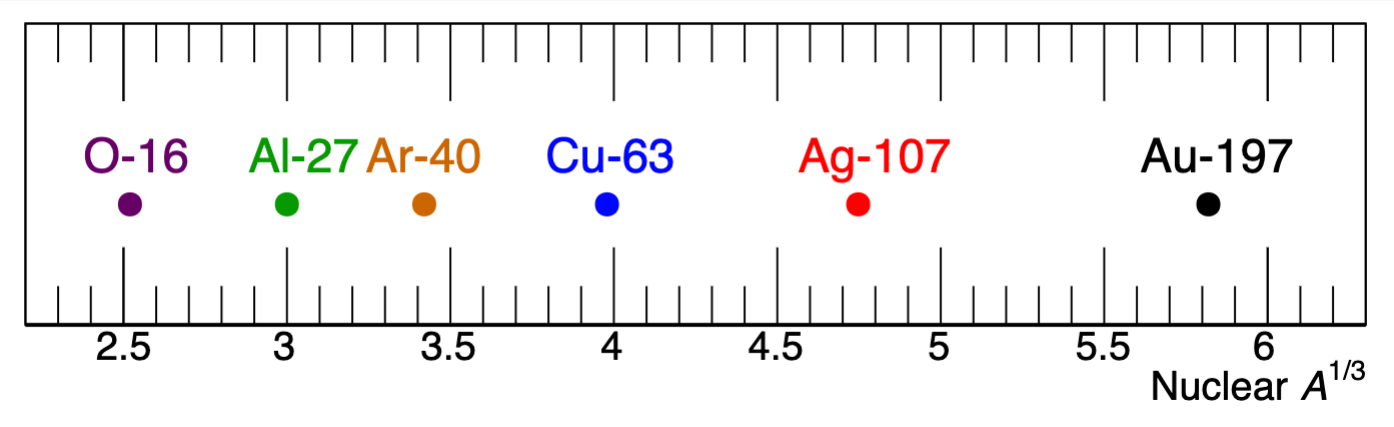
\includegraphics[width=0.85\linewidth]{figs/figure_A.png}
    \caption{Caption}
    \label{fig:figA}
\end{figure}

\begin{figure}
    \centering
    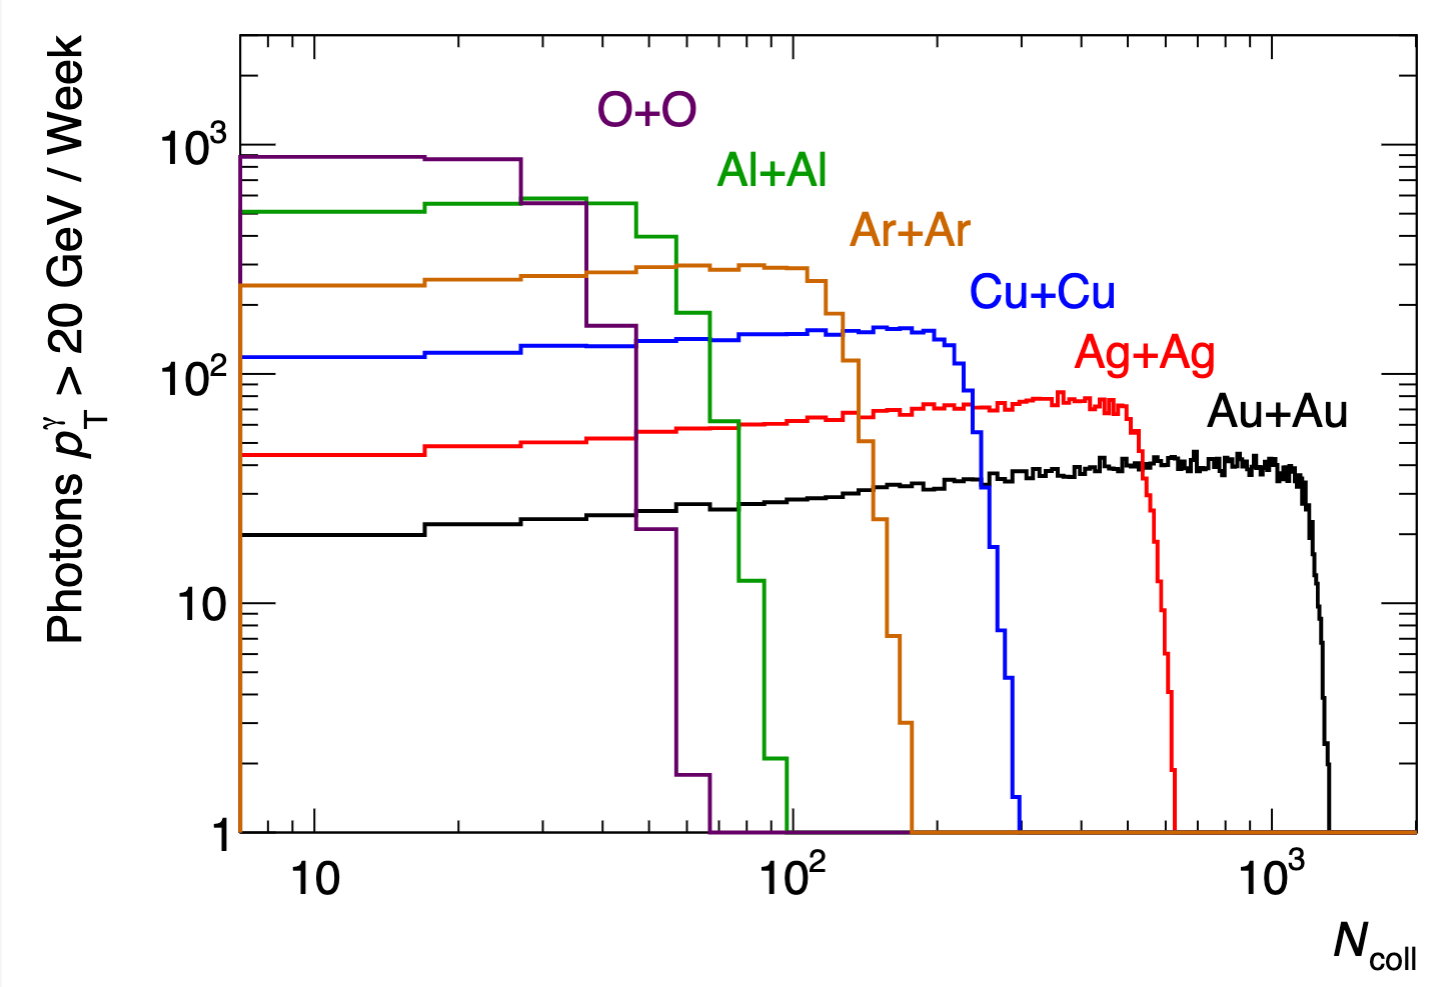
\includegraphics[width=0.85\linewidth]{figs/figure_small_perweek.png}
    \caption{Caption}
    \label{fig:figSmallPhoton}
\end{figure}


%%%%%%%%%%%%%%%%%%%%%%%%%%%%%%%%%%%%%%%%%%%%%%%%%%%%%%%%%%%%%%%%%%%%%%%%%%%%%
\newpage
\section{Cryo-Week Details}
\label{sec:cryo20262027}

In Table~\ref{tab:cryoplan2026} and Table~\ref{tab:cryoplan2027} we detail the 28 cryo-weeks of potential running in 2026 and 2027 respectively.

\begin{table}
\centering
\begin{tabular}{ | c | l | }
\hline
Weeks & Designation \\ \hline
0.5  & Cool Down from 50 K to 4 K \\ \hline
2.0  & Set-up mode 1 (p$^{\uparrow}$p$^{\uparrow}$ at 200 GeV) \\ \hline
0.5  & Ramp-up mode 1 (8 h/night for experiment) \\ \hline
15.5 & Data taking mode 1 (p$^{\uparrow}$p$^{\uparrow}$ Physics) \\ \hline
2.0  & Set-up mode 2 (O+O at 200 GeV) \\ \hline
0.5  & Ramp-up mode 2 (8 h/night for experiment) \\ \hline
2.0 & Data taking mode 2 (O+O Physics) \\ \hline
2.0  & Set-up mode 3 (Ar+Ar at 200 GeV) \\ \hline
0.5  & Ramp-up mode 3 (8 h/night for experiment) \\ \hline
2.0 & Data taking mode 3 (Ar+Ar Physics) \\ \hline
0.5  & Controlled refrigeration turn-off \\ \hline \hline \hline
28.0 & Total cryo-weeks \\
\hline
\end{tabular}
\caption{Year 2026 run plan for 28 cryo-weeks with p$^{\uparrow}$p$^{\uparrow}$, O+O, and Ar+Ar 200~GeV collisions.\label{tab:cryoplan2026}}
\end{table}


\begin{table}
\centering
\begin{tabular}{ | c | l | }
\hline
Weeks & Designation \\ \hline
0.5  & Cool Down from 50 K to 4 K \\ \hline
2.0  & Set-up mode 1 (Au+Au at 200 GeV) \\ \hline
0.5  & Ramp-up mode 1 (8 h/night for experiments) \\ \hline
24.5 & Data taking mode 1 (Physics) \\ \hline
0.5  & Controlled refrigeration turn-off \\ \hline \hline \hline
28.0 & Total cryo-weeks \\
\hline
\end{tabular}
\caption{Year 2027 run plan for 28 cryo-weeks with Au+Au 200~GeV collisions.
\label{tab:cryoplan2027}}
\end{table}